\begin{figure*}
    \centering
    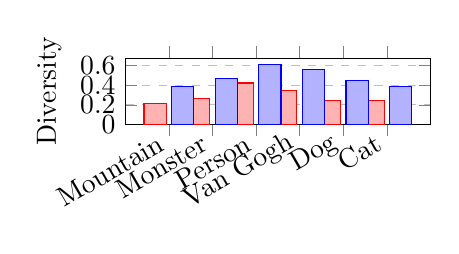
\begin{tikzpicture}[baseline, xshift=-0.3\textwidth]
    \begin{axis}[
            % Basic settings
            width=0.45\textwidth,
            height=0.2\textwidth,
            ylabel={Diversity},
            % Bar settings
            ybar=2pt,   % Gap between bars
            bar width=8pt,
            symbolic x coords={Mountain, Monster, Person, Van Gogh, Dog, Cat},
            xtick=data,
            enlarge x limits=0.2,
            % Legend settings
            legend image code/.code={%
                \draw[#1, draw=none] (0cm,0cm) rectangle (0.3cm,0.2cm);
            },
            legend style={
                at={(0.9,-0.05)},  % Position in upper right
                anchor=north west,  % Anchor point
                draw=none,         % No border
                fill=none,         % No background
                legend columns=1
            },
            % Y-axis settings
            ymin=0,
            ymajorgrids=true,
            grid style=dashed,
            % Rotated x labels
            x tick label style={
                rotate=30,
                anchor=east
            },        ]
        % Baseline method
        \addplot[red,fill=red!30] coordinates {
            (Mountain,0.217)
            (Monster,0.266)
            (Person,0.423)
            (Van Gogh,0.349)
            (Dog,0.246)
            (Cat,0.246)        };

        
        % Our method
        \addplot[blue,fill=blue!30] coordinates {
            (Mountain,0.387)
            (Monster,0.472)
            (Person,0.613)
            (Van Gogh,0.557)
            (Dog,0.444)
            (Cat,0.387)        };
        
        \end{axis}
    \end{tikzpicture}
    \hspace{0.02\textwidth}
    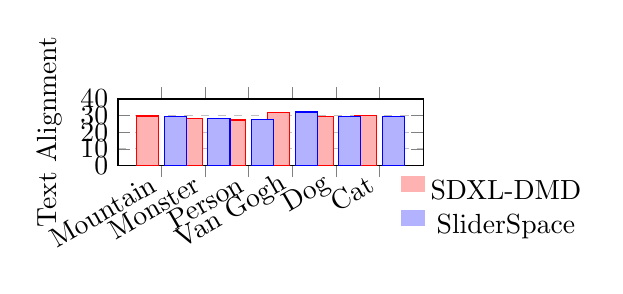
\begin{tikzpicture}[baseline, xshift=0.3\textwidth]
    \begin{axis}[
            % Basic settings
            width=0.45\textwidth,
            height=0.2\textwidth,
            ylabel={Text Alignment},
            % Bar settings
            ybar=2pt,   % Gap between bars
            bar width=8pt,
            symbolic x coords={Mountain, Monster, Person, Van Gogh, Dog, Cat},
            xtick=data,
            enlarge x limits=0.2,
            % Legend settings
            legend image code/.code={%
                \draw[#1, draw=none] (0cm,0cm) rectangle (0.3cm,0.2cm);
            },
            legend style={
                at={(0.9,-0.05)},  % Position in upper right
                anchor=north west,  % Anchor point
                draw=none,         % No border
                fill=none,         % No background
                legend columns=1
            },
            % Y-axis range
            ymin=0,
            ymax=40.0,  % Set maximum y value
            % Y-axis settings
            ymin=0,
            ymajorgrids=true,
            grid style=dashed,
            % Rotated x labels
            x tick label style={
                rotate=30,
                anchor=east
            },        ]
        % Baseline method
        \addplot[red,fill=red!30] coordinates {
            (Mountain,29.75)
            (Monster,28.14)
            (Person,27.38)
            (Van Gogh,31.94)
            (Dog,29.38)
            (Cat,29.95)        };

        
        % Our method
        \addplot[blue,fill=blue!30] coordinates {
            (Mountain,29.33)
            (Monster,28.14)
            (Person,27.40)
            (Van Gogh,32.20)
            (Dog,29.20)
            (Cat,29.20)        };
        
        \legend{SDXL-DMD, SliderSpace}
                
        \end{axis}
    \end{tikzpicture}    \caption{(left) SliderSpace generates diverse variations of a concept, as measured by DreamSim~\cite{dreamsim} distance across generated samples (higher is better). (right) The method maintains similar text-to-image alignment, as measured by CLIP Scores~\cite{hessel2021clipscore} (lower is better). }
    \label{fig:concept-diversity}
\end{figure*}